		\subsection{package kit.edu.pse.fridget.client.viewmodel}
		\begin{figure}[H]
	       \centering
	       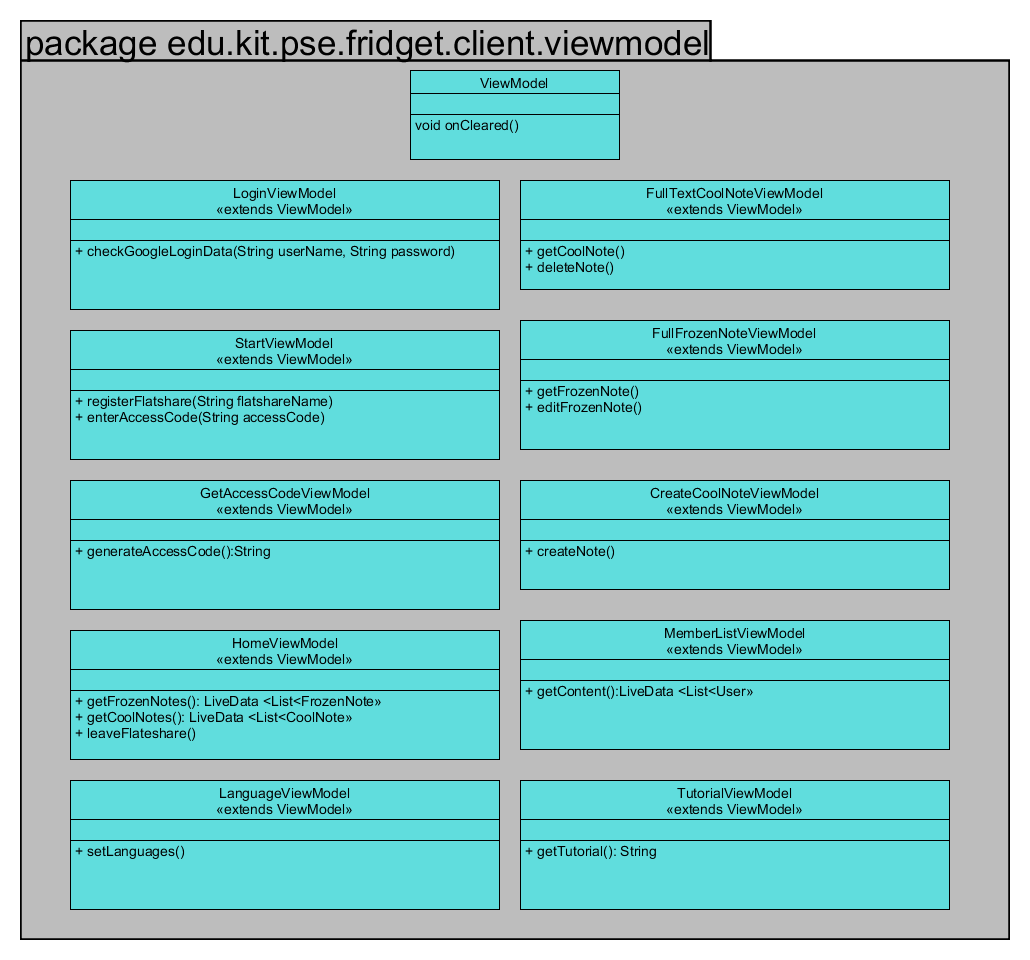
\includegraphics[scale = .35]{ViewModel.png}
	       \caption{Klassen des ViewModels}
	      \end{figure}
		\subsubsection{\texttt{public class LoginViewModel extends ViewModel}}
        \textit{LoginViewModel ist das ViewModel zur LoginActivity. In dieser Klasse wird geprüft, ob der Benutzer sich korrekt einloggt.}\\
        
		\textbf{Methoden} \\
 			\begin{itemize}
        		\item{public void checkGoogleLoginData(String userName, String password)}
        	
        		\textit{Diese Methode überprüft ob die eingegebenen Google-Daten richtig sind}
        	
        		\textbf{Parameter} \\
				userName: Google-Account Adresse

				\textbf{Parameter} \\
				password: Passwort

				\textbf{Rückgabewert} \\
				boolean: gibt an, ob die eingebenen Werte richtig oder falsch sind
   
       		 \end{itemize}
             
             	\subsubsection{\texttt{StartViewModel extends ViewModel}}
        \textit{Diese Klasse ist das ViewModel zur StartActivity, CreateFlatshareActivity, EnterAccessCodeActivity. Sie ermöglicht das Einloggen in die WG und stellt alle Daten der WG zur Verfügung.}\\
        \\
		\textbf{Methoden} \\
 			\begin{itemize}
        		\item{public void registerFlatshare(String flatshareName)}
        	
        		\textit{Diese Methode lässt eine neue WG mit dem übergebenen Namen erstellen. Dabei erstellt sie ein Objekt des Models User und übergibt diesen dem FlatShareService. Wenn in der Datenbank eine neue Flatshare angelegt wurde, erfragt diese Methode die Flatshare-ID und speichert auf einem Local Repository die FlateShare-ID sowie die User-ID.}
        	
        		\textbf{Parameter} \\
				flatshareName: Name der WG


        		\item{public void enterAccessCode(String accessCode)}
        	
        		\textit{Diese Methode lässt den AccessCode überprüfen und stellt die passenden Daten zu der WG bereit. Sobald die FlateShare-ID bekannt ist, wird sie mit der User-ID auf einem Local Repository gespeichert.}
        	
        		\textbf{Parameter} \\
				accessCode: Zugangscode
   
       		 \end{itemize}
             
             		\subsubsection{\texttt{public class GetAccessCodeViewModel extends ViewModel}}
        \textit{Diese Klasse ist das ViewModel zur GetAccessCodeActivity. Sie dient zur Generierung des Zugangscodes.}\\
        \\
		\textbf{Methoden} \\
 			\begin{itemize}
        		\item{public String generateAccessCode()}
        	
        		\textit{Diese Methode lässt einen zufälligen, einzigartigen AccessCode generieren und gibt diesen zurück.}
        	
        		\textbf{Rückgabewert} \\
				Der generierte Zugangscode wird zurückgegeben.
   
       		 \end{itemize}
             
             
            		\subsubsection{\texttt{public class HomeViewModel extends ViewModel}}
        \textit{HomeViewModel ist das ViewModel zur HomeActivity. Diese Klasse aktualisiert die Daten in der HomeActivity. Sie überprüft also, ob die Anordnung der Cool Notes verändert wurde, ob die Frozen Notes verändert wurden usw.}\\      
        \\
		\textbf{Methoden} \\
 			\begin{itemize}
        		\item{public LiveData <List<FrozenNote>> getFrozenNotes()}
        	
        		\textit{Diese Methode übergibt die Daten aller Frozen Notes auf der Pinnwand.}
        		
        		\textbf{Rückgabewert} \\
				Die Liste an Frozen Notes wird in Form von LiveData zurückgegeben.
        	
        		\item{public LiveData <List<CoolNote>> getCoolNotes()}

        		\textit{Diese Methode holt sich die Daten aller Cool Notes auf der Pinnwand sowie deren Anordnung.}
        		
        		\textbf{Rückgabewert} \\
				Die Liste an Cool Notes wird in Form von LiveData zurückgegeben.
				
				\item{public void leaveFlateshare()}
        	
        		\textit{Diese Methode sorgt dafür, dass alles, was derjenige, der die WG verlässt, erstellt hat, gelöscht wird. Außerdem wird derjenige aus der Mitgliederliste gelöscht.}
        		
       		 \end{itemize}
             
             
           		\subsubsection{\texttt{public class FullTextCoolNoteViewModel extends ViewModel}}
        \textit{Diese Klasse ist das ViewModel zur FullTextCoolNoteActivity und FullImageCoolNoteActivity. Diese Klasse verwaltet alle Daten, die für die Großansicht der Cool Note benötigt wird.}\\
        \\
		\textbf{Methoden} \\
 			\begin{itemize}
        		\item{public void getCoolNote()}
        	
        		\textit{Diese Methode holt alle Daten der CoolNote und speichert sie in einzelne Attribute, die mit den get-Methoden geholt werden können.}
        		
        		\item{public void deleteNote()}
        	
        		\textit{Diese Methode veranlasst das Löschen der Note in der Datenbank.}

       		 \end{itemize}
             
             
                 \subsubsection{\texttt{public class FullFrozenNoteViewModel extends ViewModel}}
        \textit{Diese Klasse ist das ViewModel zur FullTextFrozenNoteActivity. Dieses ViewModel holt alle benötigten Daten für die Großansicht der Frozen Note.}\\
        \\
		\textbf{Methoden} \\
 			\begin{itemize}
        		\item{public void getFrozenNote()}
        	
        		\textit{Diese Methode holt alle Daten der Frozen Note und speichert sie in einzelne Attribute, die mit den get-Methoden geholt werden können.}
        	
        		\item{public void editFrozenNote(String title, String content)}
        	
        		\textit{Diese Methode speichert die neuen Daten.}
        	
        	\textbf{Parameter} \\
				title: Überschrift
				
			\textbf{Parameter} \\
			content: Inhalt
				
       		 \end{itemize}
       		 
           		\subsubsection{\texttt{public class CreateCoolNoteViewModel extends ViewModel}}
        \textit{CreateCoolNoteViewModel ist das ViewModel zur CreateTextCoolNoteActivity und CreateImageCoolNoteActivity. Es wird benötigt, um die neu erstellten Cool Notes zu speichern.}\\
        \\
		\textbf{Methoden} \\
 			\begin{itemize}
        		\item{public void createNote()}
        	
        		\textit{Es wird ein neues Objekt CoolNote erstellt und dem passenden Service übergeben, um die CoolNote in der Datenbank hinzuzufügen. Es wird eine zufällige Position berechnet.}
        	
       		 \end{itemize}
       		 
           		\subsubsection{\texttt{public class MemberListViewModel extends ViewModel}}
        \textit{Diese Klasse ist das ViewModel zur MemberListActivity. Es holt alle Daten bezüglich der Mitglieder. d.h. Magnetfarben und Namen.}\\
        \\
		\textbf{Methoden} \\
 			\begin{itemize}
        		\item{public LiveData <List<User>> getContent()}
        	
        		\textit{Diese Methode gibt die Liste der Mitglieder zurück.}
        	
        	\textbf{Rückgabewert} \\
				Die Liste der Mitglieder wird in Form von LiveData zurückgegeben.
				
       		 \end{itemize}
       		 
       		   \subsubsection{\texttt{public class LanguageViewModel extends ViewModel}}
        \textit{Diese Klasse ist das ViewModel zur LanguageActivity.}\\
        \\
		\textbf{Methoden} \\
 			\begin{itemize}
        		\item{public void setLanguages()}
        	
        		\textit{Diese Methode ändert die Sprache der App.}
        	
       		 \end{itemize}
       		 
           		\subsubsection{\texttt{public class TutorialViewModel extends ViewModel}}
        \textit{Diese Klasse ist das ViewModel zur TutorialActivity.}\\
        \\
		\textbf{Methoden} \\
 			\begin{itemize}
        		\item{public String getTutorial()}
        		
        		\textit{Diese Methode stellt die Daten der Textinhalte zur Verfügung.}
        	
       		 \end{itemize}